\documentclass[pdftex,12pt,a4paper,twoside]{article}

\usepackage{amsfonts}
\usepackage{amsthm}
\usepackage{amsmath}
\usepackage{amscd}
\usepackage{algorithm}
\usepackage{algorithmic}
\usepackage[toc]{appendix}
\usepackage{fancyhdr}
\usepackage{graphicx}
\usepackage{multirow}
\usepackage{pdfpages}
\usepackage{setspace}       % change padding
\usepackage{verbatim}       % verb newenvironment
\usepackage{wrapfig}
\usepackage{changepage}
\usepackage{url}            % clickable links
\usepackage{newclude}       % provides include for no clearpage
\usepackage{helvet}         % font
\usepackage{lipsum}         % placeholder text
\usepackage{pgfplots}       % gantt
\usepackage{listings}       % code listings
\usepackage{array}          % default column format
\usepackage[none]{hyphenat} % No broken words
\usepackage{ifthen}         % conditionals
\usepackage{changepage}     % modify lengths
\usepackage{subfig}         % multiple images in on figure
\usepackage{multirow}       % multiple table rows
\usepackage[export]{adjustbox}
\usepackage{pgfgantt}       % Gantt chart package
\usepackage{titlesec}       % section spacing

\titlespacing*{\subsection}{0pt}{1em}{0.5em}
\titlespacing*{\subsubsection}{0pt}{1em}{0.25em}

\usepackage[backend=biber,dateabbrev=false]{biblatex}
\addbibresource{diss.bib}
\DeclareFieldFormat{url}{\newline\mkbibacro{URL}\addcolon\nobreakspace\url{#1}}
%URL on new line

\makeatletter
\let\old@lstKV@SwitchCases\lstKV@SwitchCases
\def\lstKV@SwitchCases#1#2#3{}
\makeatother
\usepackage{lstlinebgrd}
\makeatletter
\let\lstKV@SwitchCases\old@lstKV@SwitchCases

\lst@Key{numbers}{none}{%
    \def\lst@PlaceNumber{\lst@linebgrd}%
    \lstKV@SwitchCases{#1}%
    {none:\\%
     left:\def\lst@PlaceNumber{\llap{\normalfont
                \lst@numberstyle{\thelstnumber}\kern\lst@numbersep}\lst@linebgrd}\\%
     right:\def\lst@PlaceNumber{\rlap{\normalfont
                \kern\linewidth \kern\lst@numbersep
                \lst@numberstyle{\thelstnumber}}\lst@linebgrd}%
    }{\PackageError{Listings}{Numbers #1 unknown}\@ehc}}
\makeatother

% Use the margin size here to adjust text width!
\usepackage[margin=3cm]{geometry}
\usepackage{tikz}
\usetikzlibrary{shapes,arrows.meta, fit, matrix, positioning}

\tikzstyle{line} = [draw, -{Latex[length=5mm,width=3mm]}, line width=2pt]
\tikzstyle{thinline} = [draw, -{Latex[length=3mm,width=2mm]}, line width=1pt]

\tikzstyle{block} = [rectangle, draw, fill=blue!10,%black!10,
  text width=5em, text centered, rounded corners, minimum height=4em]
\tikzstyle{file} = [rectangle, draw, fill=blue!20,%black!20,
  minimum height=2em, text width=5em, text centered]
\tikzstyle{bin} = [circle, draw, fill=blue!30,%black!30,
  minimum height=3em, text width=5em, text centered, inner sep=0pt]

\tikzstyle{jblock} = [rectangle, draw, fill=red!20,%black!10,
  text width=5em, text centered, rounded corners, minimum height=4em]
\tikzstyle{jfile} = [rectangle, draw, fill=red!30,%black!20,
  minimum height=2em, text width=5em, text centered]
\tikzstyle{jbin} = [circle, draw, fill=red!40,%black!30,
  minimum height=3em, text width=5em, text centered, inner sep=0pt]

\tikzstyle{rblock} = [rectangle, draw, fill=green!20,%black!10,
  text width=5em, text centered, rounded corners, minimum height=4em]
\tikzstyle{rfile} = [rectangle, draw, fill=green!30,%black!20,
  minimum height=2em, text width=5em, text centered]
\tikzstyle{rbin} = [circle, draw, fill=green!40,%black!30,
  minimum height=3em, text width=5em, text centered, inner sep=0pt]

\tikzstyle{wfile} = [rectangle, draw, minimum height=2em, text width=5em, text centered]
\tikzstyle{wblock} = [rectangle, draw, text width=5em, text centered, rounded corners, minimum height=4em]

\fancyhf{}
\pagestyle{fancy}
\renewcommand{\headrulewidth}{0.2pt}
\renewcommand{\abstractname}{\vspace{-\baselineskip}}

% Styles can be Sonny, Lenny, Glenn, Conny, Rejne, Bjarne and Bjornstrup
\usepackage[Sonny]{fncychap}

\graphicspath{ {./figures/} }
\setlength{\parskip}{.5em}
\linespread{1.75}

\newcommand{\codelabel}[1]{
\vspace{-1em}
\begin{footnotesize}
  \hfill#1
\end{footnotesize}
}

\newcommand{\codeline}[2]{
\begin{adjustwidth}{-.5in}{-.5in}
 \begin{center}
 \lstinline{#1}

 \end{center}
\end{adjustwidth}

 \ifthenelse{\equal{#2}{}}
 {} %ignore if empty
 {
   \codelabel{#2}
 }
 \par
}

\newcommand{\pyline}[2]{
  \lstset{language=Python}
  \codeline{#1}{#2}
  \lstset{language=C}
}

\newcounter{mini}[subsubsection]

\newcommand{\minititle}[1]{\refstepcounter{mini}\vspace{\parskip}\hspace{-1\parindent}\textbf{~\themini. #1:}\\}

\newcommand{\tinytitle}[1]{\vspace{\parskip}\hspace{-1\parindent}\textbf{#1:}\hspace{3pt}}

\newcommand{\testresult}[2]{
\vspace{4pt}
\begin{adjustwidth}{-.5in}{-.5in}
  \begin{center}
   \setlength{\fboxsep}{1em}
   \fbox{%
    \parbox{\textwidth}{%
      \ifthenelse{\equal{#2}{pass}}
      {
        #1. The test is considered \textbf{\textcolor{green!20!black}{PASSED}}.
      }
      {
        #1 The test is considered \textbf{\textcolor{red!20!black}{FAILED}}.
      }
    }%
  }
  \end{center}
\end{adjustwidth}
\vspace{2pt}
}

\newenvironment{minipageparskip}
  {
   \begin{minipage}{.67\textwidth}% open the minipage
   \parskip 1em\relax% restore the value
   \parindent 1.5em\relax% restore the value
   \linespread{1.5}
  }
  {\end{minipage}}

\begin{document}

\lstset{language=C, basicstyle=\linespread{1.1}\ttfamily\footnotesize,
frame=tlbr,
backgroundcolor=\color{lightgray!15},
showspaces=false, showstringspaces=false,
commentstyle=\ttfamily\footnotesize\color{gray},
escapechar=|,
emph={
       cudaMalloc, cudaFree,
       __global__, __shared__, __device__, __host__,
       __syncthreads,
   }
}

%%TC:ignore
% !TEX root =  ../report.tex
% !TeX spellcheck = en-GB

\thispagestyle{empty}

\begin{spacing}{2}
	\begin{center}
		\includegraphics[scale = 0.45]{Preamble/WarwickCrest.pdf}
	\end{center}
	\vspace{5mm}
	\begin{center}
		\textbf{\LARGE Just In Time Compilation for a High-Level DSL}
		\vspace{5mm}
	\end{center}
	\begin{center}
		\textbf{\Large Nathan Dunne}\\
		\textbf{\large 1604486}
		\vspace{20mm}
	\end{center}
	\begin{center}
		\textbf{\Large 3rd Year Dissertation Project}\\
		\textbf{\large Supervised by Dr. Gihan Mudalige}\\
		\vspace{20mm}
	\end{center}
	\begin{center}
		{\large Department of Computer Science}\\
		{\large University of Warwick}\\
		{\large 2019--20}
	\end{center}
\end{spacing}

\pagenumbering{roman}

% !TEX root =  ../report.tex
% !TeX spellcheck = en-GB

%
\vspace*{\fill}
\begin{adjustwidth}{55pt}{55pt}

\section*{Abstract}
\addcontentsline{toc}{section}{Abstract}
The OP2 Domain Specific Language was originally developed to simplify the process of writing unstructured mesh solver applications for High Performance Computing. This report details the implementation of a new optimisation to the code generation portion of the OP2 Framework, which allows HPC applications to re-compile at run-time when the inputs to the program are known. The inputs being fixed allows for more aggressive optimisations to be applied to the program, which would not be possible at compile-time.
\par It also covers benchmarking data gathered using the new optimisation on a representative example application. The results show that if the problem size is sufficiently large, there can be benefit, however the speed-up is not significant. Further run-time optimisations are discussed that could provide further speed-up. The finished JIT compilation platform will aid in adding additional optimisations in the future.

\section*{Key Words}
\addcontentsline{toc}{section}{Key Words}
High Performance Computing, Unstructured Mesh, Just-In-Time Compilation
\end{adjustwidth}
\vspace*{\fill}

% !TeX spellcheck = en-GB

\vspace*{\fill}
\begin{adjustwidth}{55pt}{55pt}
\section*{Acknowledgements}
\addcontentsline{toc}{section}{Acknowledgements}
I am grateful for the assistance given by my project supervisor, Dr. Gihan Mudalige, for helping me develop the idea for this project, and guiding me throughout with his expertise in the field. This gratitude should extend to all teaching staff at the University of Warwick Computer Science Department, for inspiring me throughout my degree.
\par Special thanks must also go to the Cambridge Service for Data-Driven Discovery , for allowing me to use their machines to gather benchmarking data for my implementation.
\par Finally, I wish to acknowledge the help provided by Yvette Dunne, Rachel Dunne, and Kaviyana Sitartha in reading over many pages of drafts, and providing much needed feedback.
\end{adjustwidth}
\vspace*{\fill}

% !TeX spellcheck = en-GB

\tableofcontents
\listoffigures

% !TeX spellcheck = en-GB

\pagenumbering{arabic}

\lfoot{\centering \thepage}

%%TC:endignore

% !TEX root =  ../report.tex
% !TeX spellcheck = en-GB

\section{Introduction}
%The introduction should provide content for the report, discuss relevant background material and state the main aims of the work. Clearly establishing the aims of the work is important for this coursework, since you have a great deal of freedom in what you will seek to achieve.

In the field of High Performance Computing (HPC), computers with processing power hundreds of times greater than conventionally available machines are used to solve or approximate complex problems. Such systems almost always utilize parallelism, which involves multiple processing units working simultaneously on a single problem, to find solutions within a tractable time.
\par Many paradigms for executing parallel workloads have emerged over time. Recently, General Purpose Graphical Processing Units (GPUs) have become an increasingly popular hardware architecture, having originally been conceived as specialised hardware for graphical shader calculations. GPU's high number of parallel processing units allow a high degree of parallelism, as well as being able to execute operations usually done by the CPU. Passing compute-heavy workloads to a GPU device can lead to significant speed-ups over sequential execution, and remove the CPU as a bottleneck.
\par
Commonly, a single developer or team is unlikely to have both the necessary expertise in a niche area of physics with a non-trivial problem to be solved; and also sufficient depth of knowledge in computer science to understand the latest generation of parallel hardware. For this reason the OP2 framework was created: to provide a high level abstraction in which HPC applications can be written, and separate the application code from the optimisation requirements. OP2 is already able to generate optimised code for a number of back-ends from an application file.
\par
This report details an investigation into implementing and benchmarking a new optimisation to the GPU code generation in OP2. The optimisation is named ``Just-In-Time (JIT) Compilation" for its similarities to a comparable process often performed by compilers when run-time efficiency is desired. All compilation that takes place prior to run-time is referred to as ``Ahead-Of-Time (AOT) Compilation".
\vfill
\subsection{Motivations}
The idea for this project was provided by my supervisor, Dr Gihan Mudalige - an Associate Professor in the University of Warwick Computer Science Department. It was pulled from the pool of uncompleted features for the OP2 project, and was selected because it aligned with my interest in High Performance Computing, and previous experience with optimising existing codes.
\par
Since OP2 is Open Source and freely available, the implementation I produce will become part of the framework, allowing future contributors to build on my work.

\subsection{Background Work}
\label{s:bgwork}

In order to become comfortable with the OP2 framework and provide a useful contribution, it is important to understand the domain of problems for which it was created: Unstructured Mesh Solvers.
\par
A large proportion of HPC workloads involve approximating Partial Differential Equations (PDEs) to simulate complex interactions in physics problems, for example the Navier-Stokes equations for computational fluid dynamics, or predicting weather patterns. It is usually necessary to discretise such problems, which means dividing a continuous space into a number of discrete cells such as in Figure \ref{fig:2dmesh}.\par
\begin{figure}[h!]
  \begin{minipage}{.5\textwidth}
    \centering
    \begin{tikzpicture}[x=2.6ex, y=2.6ex]
      \draw (0,6) -- (0,3) -- (5,3) -- (5,0) -- (8,0) -- (8,2) -- (9,2) -- (9,6) -- (8,6) -- (8,7) -- (4,7) -- (4,6) -- cycle ;
    \end{tikzpicture}
  \end{minipage}
\begin{minipage}{.5\textwidth}
  \centering
  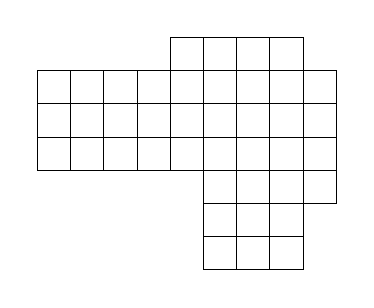
\begin{tikzpicture}
  \tikzset{
    square matrix/.style={
      matrix of nodes,
      column sep=-\pgflinewidth, row sep=-\pgflinewidth,
      nodes={
        rectangle,
        draw=black,
        minimum height=#1,
        anchor=center,
        align=center,
        text width=#1,
        text height=2ex,
        text depth=0.5ex,
        inner sep=0pt,
      }
    },
    square matrix/.default=1.2em
  }

  \matrix[square matrix]
  {
  &&&&                    $ $ & $ $ & $ $ & $ $ \\
  $ $ & $ $ & $ $ & $ $ & $ $ & $ $ & $ $ & $ $ & $ $ \\
  $ $ & $ $ & $ $ & $ $ & $ $ & $ $ & $ $ & $ $ & $ $ \\
  $ $ & $ $ & $ $ & $ $ & $ $ & $ $ & $ $ & $ $ & $ $ \\
  &&&&&                         $ $ & $ $ & $ $ & $ $ \\
  &&&&&                         $ $ & $ $ & $ $ \\
  &&&&&                         $ $ & $ $ & $ $ \\
  };

  \end{tikzpicture}
  \end{minipage}
  \caption{Example 2D decomposition}
  \label{fig:2dmesh}
\end{figure}
\noindent Depending on its structure, a mesh can be described as either structured (regular) or unstructured. Structured meshes such as in Figure \ref{fig:struct} are made up of cells following a regular pattern, while unstructured meshes use connectivity information to specify the mesh topology, as in Figure \ref{fig:umesh}.
\vspace{.5cm}
\begin{figure}[h!]
  \begin{minipage}{.5\textwidth}
    \centering
    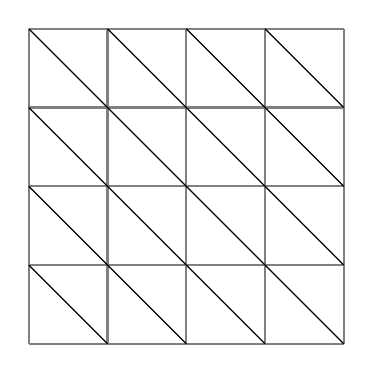
\begin{tikzpicture}
      \draw[step=1cm,gray,thick]
      (0,0) grid (4,4);

      \foreach \x in {0,...,3}{
        \draw (\x, 0) -- (0, \x) ;
        \draw (\x, 4) -- (4, \x) ;
      }

    \end{tikzpicture}
    \caption{Tri-Structured Mesh}
    \label{fig:struct}
  \end{minipage}
  \begin{minipage}{.5\textwidth}
    \centering
    \includegraphics[width=.55\textwidth]{umesh}
    \caption{Airfoil Tri-Unstructured Mesh}
    \label{fig:umesh}
  \end{minipage}
\end{figure}
\par
\noindent A particular simulation might, for example, be approximating the velocity of a fluid in each cell, and at every time step re-calculate this value based on the values of cells around it. A program utilising a structured mesh will make use of a repeating pattern to calculate values, which is commonly referred to as a `stencil code' \cite{stencil}. An example of a 2D stencil is shown in Figure \ref{fig:stencil}.\par
\vspace{.5cm}
\begin{figure}[h!]
  \centering
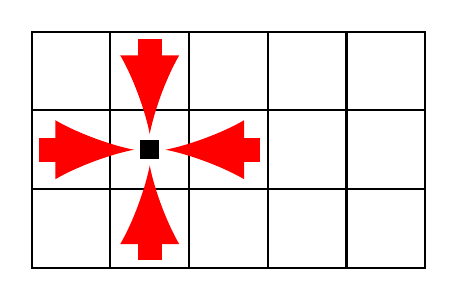
\begin{tikzpicture}

\foreach \x in {0,...,4}{
  \foreach \y in {0,...,2}{
    \node [fill=none, draw=black, thick, minimum size=1cm]
      at (\x+.5, \y+.5) {};
  }
}

\node [fill=black] at (1.5, 1.5) {};

\draw[->,>=latex, red, line width=3mm] (0.1,1.5) -- (1.3,1.5);
\draw[->,>=latex, red, line width=3mm] (2.9,1.5) -- (1.7,1.5);
\draw[->,>=latex, red, line width=3mm] (1.5,0.1) -- (1.5,1.3);
\draw[->,>=latex, red, line width=3mm] (1.5,2.9) -- (1.5,1.7);

\end{tikzpicture}
\caption{Example 2D stencil code}
\label{fig:stencil}
\end{figure}
\noindent Unstructured meshes cannot use a stencil as the underlying mesh is irregular, so instead they must use indirect array accesses where a value retrieved from one array is used to index another array. When a value is updated, multiple levels of memory reference indirection will be involved, as a list of neighbouring points must be obtained, and their values loaded \cite[p10]{berkley}. This is much more computationally intensive that accessing data using a stencil.

\clearpage
\subsection{Report Structure}
The rest of this report is structured as follows: In Section \ref{s:research} (p\pageref{s:research}) the research done to inform the work in this project is discussed, along with relevant similar academic work. This is followed by a Project Specification in Section \ref{s:spec} (p\pageref{s:spec}), which includes the requirements of the project, and a high level plan of the implementation to be completed, its components, and how they will interact.
Section \ref{s:impl} (p\pageref{s:impl}) details the Implementation itself, and the expected results of code generation with JIT compilation enabled, and Section \ref{s:test} (p\pageref{s:test}) explains the plan for, and outcome of, Testing and Benchmarking using an example application on a HPC cluster.
\par Section \ref{s:eval} (p\pageref{s:eval}) contains an Evaluation of the work completed, including a discussion of Future Work (p\pageref{ss:fw}) which could build on top of what was done for this report; and a reflection on Project Management (p\pageref{ss:pm}). Lastly, Section \ref{s:conc} (p\pageref{s:conc}) provides an overall Conclusion.

% !TEX root =  ../report.tex

\section{Research}

\subsection{OP2}
\par
The OP2 library is already able to generate optimised code for a number of platforms, including the increasingly popular NVidia CUDA for parallel programming on NVidia GPUs. The current implementation is compiled entirely ahead of time however, and is not able to optimise based on the input mesh.
\par
The abstraction provided by OP2 allows scientists and engineers to focus on the description of the problem, and seperates the consideration for parallelism and efficiency into the back-end library and code generation.
This is beneficial as it is unlikely that a single developer or team has the necessary expertise in both some niche area of physics with a non-trivial problem to be solved; and sufficient depth of knowledge in computer science to understand and utilise the latest generation of parallel hardware.
\par
A further benefit is that existing solutions which make use of the OP2 library can be ported onto a new generation of hardware, by modifying only the OP2 backend library to support the new hardware, instead of every application individually. This portability can save both time and money in development if multiple different hardware platforms are desired to be used.


\subsection{CUDA}

\subsection{Related Work}

\subsubsection{JIT}
\label{sec:rw_JIT}

\subsubsection{Similar Libraries}

% !TEX root =  ../report.tex
% !TeX spellcheck = en-GB

\section{Specification}
\label{s:spec}

In order to clearly explain the design of the extension that will be made to the OP2 framework, it is important to first understand the existing work-flow. The following is a high level overview of the components of OP2 that pre-date this project, so that when the new system is described in Section \ref{ss:reqs} it is easier to understand.

\subsection{Existing System}
\begin{figure}[h!]
\makebox[\textwidth][c]{
 \resizebox{1.1\textwidth}{!}{
  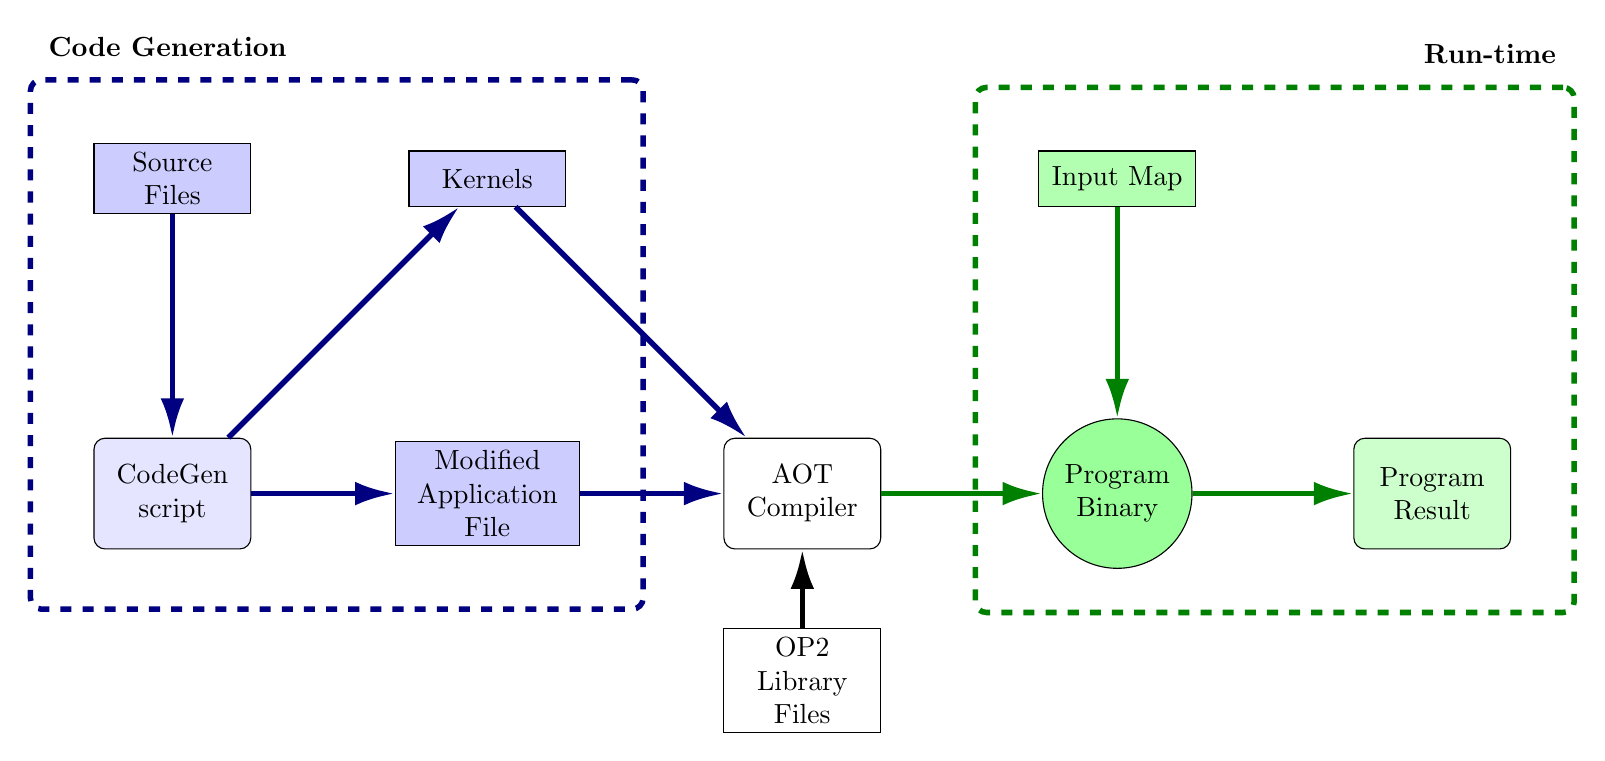
\begin{tikzpicture}[node distance=4cm, auto]
    \node [file] (source) {Source Files};
    \node [block, below of=source] (op2py) {CodeGen script};
    \node [file, right of=op2py, text width=6em] (sourceOp) {Modified Application File};
    \node [file, above of=sourceOp] (Kernels) {Kernels};
    \node [wblock, right of=sourceOp] (aot) {AOT Compiler};
    \node [wfile, below=1cm of aot] (op2lib) {OP2 Library Files};

    \node [rbin, right of=aot] (binary) {Program Binary};
    \node [rfile, above of=binary] (input) {Input Map};
    \node [rblock, right of=binary] (result) {Program Result};

    \tikzset{dotted box1/.style={draw=black!100, dash pattern=on 4pt off 4pt,
      inner sep=8mm, rectangle, rounded corners, line width=2pt}};

    \node (run-time) [dotted box1, fit = (input) (result), color=green!50!black] {};
    \node at (run-time.north east) [above left=2mm] (rtbox) {\textbf{Run-time}};

    \node (code-gen) [dotted box1, fit = (source) (sourceOp), color=blue!50!black] {};
    \node at (code-gen.north west) [above right=2mm] (rtbox) {\textbf{Code Generation}};

    \path [line, color=blue!50!black] (source) -- (op2py);
    \path [line, color=blue!50!black] (op2py) -- (sourceOp);
    \path [line, color=blue!50!black] (op2py) -- (Kernels);
    \path [line, color=blue!50!black] (sourceOp) -- (aot);
    \path [line, color=blue!50!black] (Kernels) -- (aot);
    \path [line, color=black] (op2lib) -- (aot);
    \path [line, color=green!50!black] (aot) -- (binary);
    \path [line, color=green!50!black] (input) -- (binary);
    \path [line, color=green!50!black] (binary) -- (result);

  \end{tikzpicture}
  }}
  \caption{Existing OP2 System Diagram}
  \label{fig:aot_sys}
\end{figure}

The pre-existing OP2 workflow is shown in Figure \ref{fig:aot_sys}. The diagram starts in the top left with the Code Generation stage, beginning at the system's input: a set of Source Files. The set of Source Files cannot be empty, and must contain at least one file, called the Master Application file. The Master Application file is a normal C program, containing OP2 API calls to define of sets, maps, and constants, as well as initialising and cleaning up the OP2 execution with the \verb|op_init()| and \verb|op_exit()| Library functions. It describes the structure of the application.
\par
The input Source Files can optionally contain addition C source and header files, included in the normal way with \verb|#include| statements, to assist with the organisation of a complex application with a large code-base. An example usage of these files would be a header file for each parallel loop, containing the function to be executed as the body of the loop.
\par
These Source files are parsed by the code generation Python script, from which the output is: a modified version of the master application file, and a kernel file for each parallel loop. The output files are compiled, and linked against the OP2 library files for the desired hardware platform to produce an executable Program Binary. The expectation is that this binary will run without error on the target hardware, taking a map as an input to produce the result desired by the application programmer.
\par
The existing system is able to generate optimised code for the target platform from the high level application code, and apply compiler optimisations ahead of time, including optimisations like \verb|-O3| and \verb|--use_fast_math|. It is not, however, able to optimise based on the inputs at all, as they are only known at runtime, after the compiler has completed and the binary is being executed. This is where the implementation for this project comes in: to provide the ability to use the input data when optimising.

\subsubsection{op2.py}
\label{ss:impl_op2}
The code generation is done using Python scripts, with the main script being \verb|op2.py|, which parses the input files to gather data, and provides this data to a number of other scripts, which each perform the code generation for a specific hardware platform. It uses the Python Regular Expressions (RegEx) library: \verb|re| \cite{re} to identify OP2 API calls in the Application File, and ensures certain conditions are met - for example that \verb|op_init| and \verb|op_exit| are both called at least once to initialise and clean up the OP2 execution environment.
\par
It also gathers information about each parallel loop, including the number of the parameters and their types, and the details of the indirect data set if the loop is indirect. This stage includes some error checking, by ensuring types and dimensions are consistent throughout the application.
\par
Once the Application has been analysed, \verb|op2.py| produces a modified copy of the Application File, named \verb|[application]_op.cpp|, which is largely the same as the file provided by the application programmer, but with the addition of \verb|extern| declarations for the function each parallel loop will call: \verb|op_par_loop_[name]|. Defining a function \verb|extern| means it has external linkage, and therefore the definition of the function may be found during the linking stage of compilation, not in the current pass.
\par
The generator scripts for each platform will receive the list of loop details gathered using RegEx as its parameters, then generates a definition of each parallel loop's execute function will be generated for each hardware platform, in the form of Kernel files. At compile time these Kernel files will be linked to the extern definition in the Modified Application File by the linker.
\par
The requirements for the code generation script that will be created as part of this project to produce kernels containing CUDA code with JIT compilation, will discussed in the following section.

\subsection{New System Requirements}
\label{ss:reqs}

Implementing the new system will require work in two main areas: a new Python code generation script, and some modifications to the OP2 library itself. The OP2 Library is currently implemented in both C and Fortran, but only the C library will be modified, due to developer familiarity with the C language. OP2 does also include code generation using MatLab, however the Python script is preferable for new developments, since Python is now ubiquitous, and provides very convenient string manipulation capabilities. The following are the necessary requirements to consider this project a success.

\subsubsection{Python Script}
The new code generation script will be named \verb|op2_gen_cuda_jit.py|, and will need to perform a somewhat similar source-to-source translation process to pre-existing CUDA script for Ahead-of-Time compiled code. The extension required is the ability to also generate a second, altered code-base that will be compiled at run-time, as well as the original code that is compiled prior to running the executable.
\par
All code generated by the new code generation script must form valid C files, and compile using a the Intel C compiler \cite{icc} without errors. Since the project will involve generation of NVidia CUDA as well, the generated CUDA code must also be valid, and compile with the NVidia C Compiler (\verb|nvcc|) from the NVidia CUDA Toolkit \cite{nvcc,toolkit} without errors.
\par
When the resulting executable has been compiled from the generated code is executed, it will need to invoke a re-compilation stage while it is running, and execute code that has been compiled during its runtime as part of its execution. It must produce an output within some tolerance of the expected result, obtained from executing the parallel loop iterations sequentially in an arbitrary order. The order is not significant, as OP2 enforces a restriction that the order in which elements are processed must not affect the final result, within the limits of finite-precision floating-point arithmetic \cite[p3]{op2main}. There cannot be any dependencies between iterations in the application, otherwise the result may vary when translated by OP2. This constraint allows the OP2 code generator the freedom to not consider the ordering of iterations, and instead select an ordering based on performance.
\par
Lastly, the above requirements must be met for both Array-of-Structs and Struct\\-of-Arrays data layouts, especially when automatic SoA conversion is enabled, as this alters the generated code.

\subsubsection{Run-time Assertions}
The application's input will be a large number of data points forming an unstructured mesh which it will operate over. The optimisation that will be made for this project is "Constant Definition", built on the assertion that values declared as OP2 constants are certainly not going to change during the course of execution. To apply this optimisation, constant values provided as part of the input must be turned into \verb|#define| directives for the C Pre-processor in the recompiled code. This will result in all references to the variable's identifier in the code being transformed so they are seen as a literal value rather than a memory read by the compiler.
\par
An example of how this is normally used can be seen in the CUDA example program from before (Appendix \ref{app:cudaEx}), where the size of the arrays to be added together is defined as \verb|N|, and everywhere \verb|N| appears in the code the literal value \verb|32| will be substituted before compilation.
\par
As a result of the need to store constant values in memory being removed, retrieval time from memory when a constant value is required has been eliminated. The literal value is immediately available. Other possible optimisations will be discussed in Section \ref{ss:fw} (Future Work).
\par
The overall goal of this project is to investigate whether this technique does provide any performance benefit, however any performance increase that incurs unacceptable deviation from the expected result is not a useful benefit. Therefore, the addition of defined constants should not reduce the accuracy of the result outside tolerance. It is not expected that it will.


\subsubsection{OP2 Library}
Outside the code generation script, some OP2 API functions may need to be implemented differently in the OP2 library files, as the functions may require additional information to be stored and retrieved at runtime. It is a requirement that the OP2 API itself is not altered in any way by modifications to the library, so that all existing programs currently using the API will be able to seamlessly update to using the modified version.

\subsection{Testing \& Benchmarking}
Once the code generation stage has been completed, and the Python Script is able to generate valid C and CUDA code that can be compiled without error for an example OP2 Application, the resulting binary needs to be tested to ensure the result is correct, and benchmarked to determine if there is performance gain. The easiest thing to compare to performance against is the same application generated for graphics cards, without JIT compilation, and see if there is any benefit. Benchmarking results will include the time taken to recompile at runtime for the JIT compiled version, and the time taken to copy constant values to device memory for the AOT compiled version.

\clearpage
\subsection{New System Model}

\begin{figure}[h!]
\makebox[\textwidth][c]{
\resizebox{1.1\textwidth}{!}{
  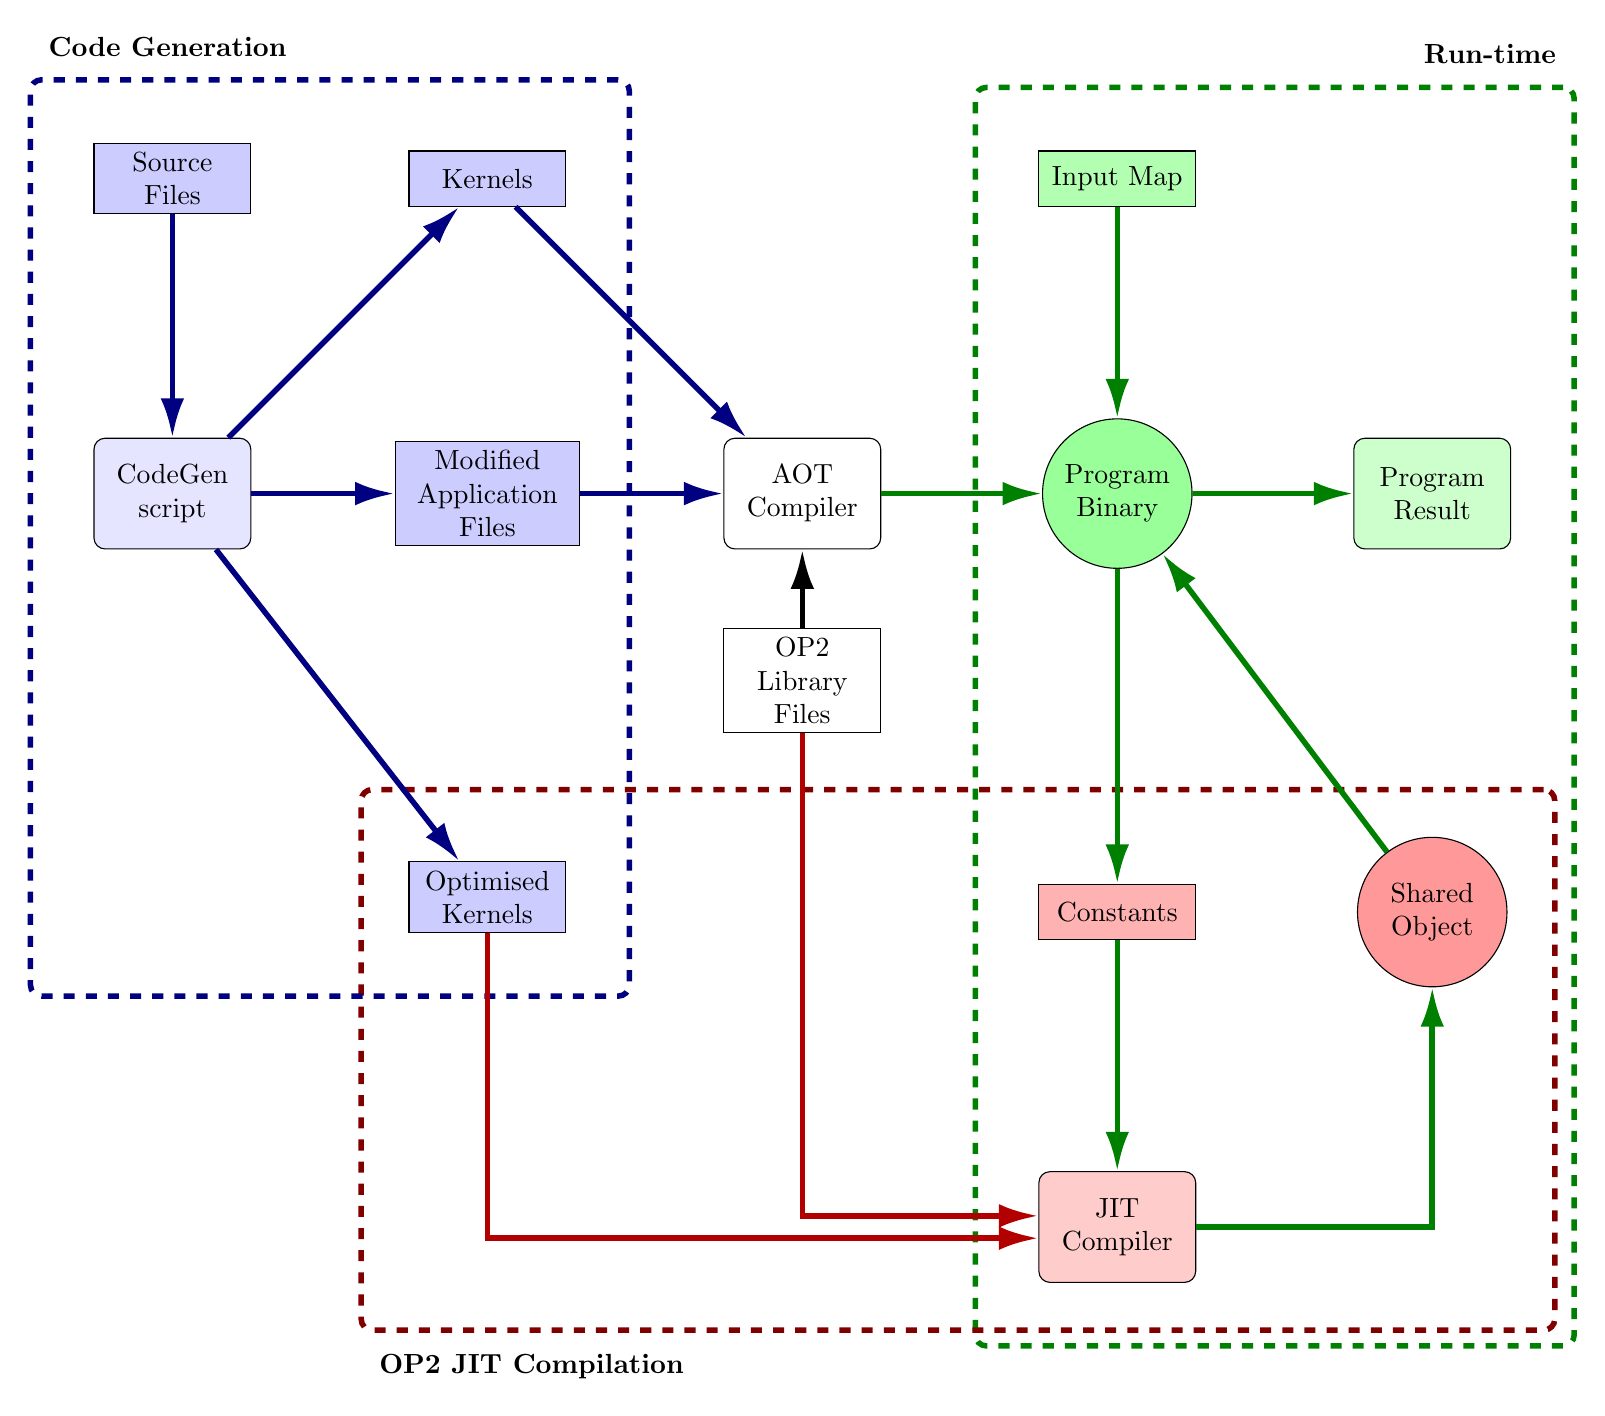
\begin{tikzpicture}[node distance=4cm, auto]
    \node [file] (source) {Source Files};
    \node [block, below of=source] (op2py) {CodeGen script};
    \node [file, right of=op2py, text width=6em] (sourceOp) {Modified Application Files};
    \node [file, above of=sourceOp] (Kernels) {Kernels};
    \node [wblock, right of=sourceOp] (aot) {AOT Compiler};
    \node [wfile, below=1cm of aot] (op2lib) {OP2 Library Files};

    \node [rbin, right of=aot] (binary) {Program Binary};
    \node [rfile, above of=binary] (input) {Input Map};
    \node [rblock, right of=binary] (result) {Program Result};

    \node [file, below=4cm of sourceOp] (recKernels) {Optimised Kernels};
    \node [jfile, below=4cm of binary] (consts) {Constants};
    \node [jblock, below of=consts] (jit) {JIT Compiler};
    \node [jbin, right of= consts] (so) {Shared Object};

    \tikzset{dotted box1/.style={draw=black!100, dash pattern=on 4pt off 4pt,
      inner sep=8mm, rectangle, rounded corners, line width=2pt}};
    \tikzset{dotted box2/.style={draw=black!100, dash pattern=on 4pt off 4pt,
      inner sep=6mm, rectangle, rounded corners, line width=2pt}};

    \node (run-time) [dotted box1, fit = (input) (jit) (result), color=green!50!black] {};
    \node (jitbox) [dotted box2, fit = (recKernels) (so) (jit), color=red!50!black] {};

    \node at (run-time.north east) [above left=2mm] (rtbox) {\textbf{Run-time}};
    \node at (jitbox.south west) [below right=2mm] (corner) {\textbf{OP2 JIT Compilation}};

    \node (code-gen) [dotted box1, fit = (source) (recKernels), color=blue!50!black] {};
    \node at (code-gen.north west) [above right=2mm] (rtbox) {\textbf{Code Generation}};

    \path [line, color=blue!50!black] (source) -- (op2py);
    \path [line, color=blue!50!black] (op2py) -- (recKernels);
    \path [line, color=blue!50!black] (op2py) -- (sourceOp);
    \path [line, color=blue!50!black] (op2py) -- (Kernels);
    \path [line, color=blue!50!black] (sourceOp) -- (aot);
    \path [line, color=blue!50!black] (Kernels) -- (aot);
    \path [line, color=black] (op2lib) -- (aot);
    \path [line, color=red!70!black] (op2lib) |- ($(jit.west)!0.2!(jit.north west)$);
    \path [line, color=green!50!black] (aot) -- (binary);
    \path [line, color=green!50!black] (input) -- (binary);
    \path [line, color=green!50!black] (binary) -- (consts);
    \path [line, color=red!70!black] (recKernels) |- ($(jit.west)!0.2!(jit.south west)$);
    \path [line, color=green!50!black] (consts) -- (jit);
    \path [line, color=green!50!black] (jit) -| (so);
    \path [line, color=green!50!black] (so) -- (binary);
    \path [line, color=green!50!black] (binary) -- (result);

  \end{tikzpicture}
  }}
  \caption{OP2 System Diagram with JIT Addition}
  \label{fig:jit_sys}
\end{figure}

\noindent Figure \ref{fig:jit_sys} describes the new workflow of the OP2 library, with Just-In-Time compilation. As before, code generation takes an input of the application and optional additional files, and generates the Kernels and Modified Application Files. It also generates an additional set of Optimised Kernels, which contain code that are only be compiled inside the green box denoting `run-time', at which point the constants from the Input Map are known to the program. These Kernel files are not seen by the ahead of time compiler.
\par
The JIT compiler also needs to link the Optimised Kernels against the OP2 Library Files, so it is necessary that they are stored in a location that is also accessible at run-time, not just when the executable is compiled. This compilation will take place during the execution of the binary, and will therefore make up part of the program's execution duration. It will result in a Shared Object or Dynamically Loaded Library (DLL) file, with a standardised name, which the program can load, and utilise the functions it makes available.
\par
The exported functions will be the recompiled versions of each parallel loop, which as black boxes are equivalent (i.e.\ they have the same inputs and outputs), however theoretically they are faster to execute than the original versions.
\par
The Kernels compiled Ahead of Time could be altered such that their sole purpose is to invoke the compiler at runtime, then pass execution over to the JIT compiled function. It could be beneficial, however, to allow executables with the JIT compilation feature enabled or disabled to be compiled from the same source code. This requires the Ahead of Time Kernels to have retain the ability to execute the loop body without requiring JIT compilation, as well as being able to initiate the runtime compilation of the optimised kernels. Therefore the compiler invocation will be wrapped in a pre-processor conditional, so that the feature can be enabled or disabled using a compiler argument: \verb|-DOP2_JIT|.

\subsection{Library Modifications}
In the OP2 library, the main API function that will need to be modified is:
\codeline{void op_decl_const(int dim, char *type, T *dat, char *name)}{\cite[p9]{manual}}
\noindent This function is used to declare a constant value, its dimension, data type, and identifier.
Previously, this function copied the value to a device symbol, so that when required it could be read from device memory. In this implementation, it needs to maintain a de-duplicated list of identifiers, and persist their values, data types, and dimensions. These parameters will be used when the first parallel loop is invoked to generate the header file. At this point it is known that no more constants can be declared. In the header file each of the constant values will have a \verb|#define| directive making the value available as a literal value.

\vspace{4em}
\noindent In the next section, the completed Implementation is discussed. The contents of the files generated by the Python code generation script will be examined in more detail, and design decisions made will be explained. The Implementation is presented in its finished form, however the development process is covered later, in Section \ref{ss:pm}.

% !TEX root =  ../report.tex

\section{Implementation}
The OP2 library is hosted open source on GitHub\cite{OP2rep}. Instructions for obtaining the implementation completed for this report, and getting started with OP2 can be found in Appendix \ref{app:getStart}.
\par
The feature branch for this project, \verb|feature/jit| was branched from \\\verb|feature/lazy-execution| on 13th November 2019. The \verb|laxy-execution| branch's last commit was in April 2018, and lagged behind the \verb|master| branch somewhat. It was rebased onto \verb|master| before any other changes were made.
\par
The \verb|lazy-execution| branch contained the beginnings of a system to execute parallel loops when values are required rather than when called. This is done through an internal library function:
\codeline{void op_enqueue_kernel(op_kernel_descriptor *desc)}{op2/c/src/core/op\_lazy.cpp [71-89]}
Which currently simply executes the function straight away. This process for calling parallel loops is used similarly throughout work done to enable Just In Time Compilation for CUDA, so that future efforts towards lazy execution can continue in the future on top of the JIT implementation.

\subsection{Code Generation}
The Python code generation script which forms the main body of the implementation can be found in: \verb|translator/c/python/jit/op2_gen_cuda_jit.py|
\\
The main function is:
\pyline{def op2_gen_cuda_jit(master, date, consts, kernels)}{translator/c/python/jit/op2\_gen\_cuda\_jit.py [102]}
Which is called from \verb|op2.py| in the parent directory - the same as the other code generation scripts. It's parameters are:\\
\begin{tabular}{>{\bfseries}l l}
  master: & The name of the Application's master file \\
  date: & The exact time of code generation \\
  consts: & list of constants, with their type, dimension and name \\
  kernels: & \parbox[t]{.8\textwidth}{list of kernel descriptors, where each kernel is a map containing many fields describing the kernel, which may alter the way the code for that loop is generated.}
\end{tabular}

% !TEX root =  ../report.tex
% !TeX spellcheck = en-GB

\section{Testing}
\label{s:test}
Throughout development, an example application that was previously developed using the OP2 API was used to test code generation, and verify the results. The application is called \textit{airfoil}, and it has been used for validating generated OP2 code before \cite{gpudesign}, as it makes use of all the key features including having both direct and indirect loops.
\par
\textit{airfoil} is a computational fluid dynamics application which models the air flow around an aeroplane wing, using unstructured grid to discretise the space. A document detailing the \textit{airfoil} code is available on the OP2 website \cite{airfoil}. Figure \ref{fig:airfoil_mesh} is an simple 120 x 60 mesh for \textit{airfoil}, showing the wing shape, and increasing granularity close to the shape. Each quadrilateral represents a cell.\par
\begin{figure}[h!]
  \centering
  \includegraphics[width=.55\textwidth]{airfoil}
\caption{Rendering of an \textit{airfoil} mesh. Diagram from \cite{gpudesign}}
\label{fig:airfoil_mesh}
\end{figure}
\par
\vfill
\noindent To ensure that the test cases selected definitely validate the implementation, the requirements set out in the Specification must be revisited. They are summarised in the next Section.
\clearpage
\subsection{Requirements}
  \begin{outline}[enumerate]
  \1 Source code files must be produced as the output of the new code generation Python script.
  \1 The generated source code files must be valid.
  \2 C code must compile using \verb|icc| without errors;
  \2 CUDA code must compile with \verb|nvcc| without errors.
  \1 The compiled executable must invoke a re-compilation stage, if the feature is enabled.
  \2 Re-compilation must also complete without error;
  \2 The binary must execute code that has been compiled during its execution.
  \1 Constant values from the input must be available to the User Function.
  \2 If JIT is enabled, they must be turned into \verb|#define| directives;
  \2 Otherwise they must be copied to device memory.
  \1 The compiled executable must produce a result within some tolerance of the expected result.
  \1 The OP2 API must not be modified.
  \end{outline}

\noindent Section \ref{ss:results} is the final results of the test plan used throughout the project whenever a work done needed to be validated. Each test  ensures that a requirement from the above list has been met, and also includes the date when it first passed.
\par
Requirement 6 can be trivially accepted when testing, since the implementation did not modify the OP2 API. There is no test for this requirement.

\subsection{Initial State}
\begin{wrapfigure}[18]{l}{0.45\textwidth}
  \centering
\caption{\textit{airfoil} folder initial state}
\label{fig:files_a}
\includegraphics[width=0.4\textwidth]{files1}
\end{wrapfigure}
The initial state for testing is a folder containing the source files for \textit{airfoil}, as listed in Figure \ref{fig:files_a}. The Application File is \verb|airfoil.cpp|, and the five header files each contain a User Function for the parallel loop with the same name.
\par
\verb|new_grid.h5| is the name of the input data file, formatted in the Heterogeneous Data Format (HDF5) \cite{HDF5}. This file can be obtained from the OP2 website \cite{op-dsl}, and must be converted from \verb|.txt| to \verb|.h5| using the \verb|convert_mesh| tool.
\par
OP2 already provides a standard set of functions for performing file I/O on an HDF5 file, which \textit{airfoil} uses. The contents of the file can be viewed using the \verb|hdump| utility, which comes with an HDF5 installation.

\clearpage
\subsection{Test Plan \& Results}
\label{ss:results}

\hspace{\parindent}\minititle{``Source code files must be produced as the output of the new code generation Python script."}
To test the code generation, the python script \verb|op2.py| is called in the directory, passing the main application file \verb|airfoil.cpp| as an argument, as well as the string \verb|JIT| to make sure the correct GPU code generation script is used. \par
The environmental variable \verb|$OP2_INSTALL_PATH| can be assumed to hold to full path to the \verb|op2/| folder in the top level of the OP2 repository. Since the translation script is in a sub-directory of \verb|translator/|, which is also a top-level folder, the path to the Python translator script will be as shown below.
\codeline{> python2 \$OP2_INSTALL_PATH/../translator/c/python/op2.py airfoil.cpp JIT}{}

\noindent After running this command in the \textit{airfoil} directory, the expected outcome is that a new file: \verb|airfoil_op.cpp| is created, as well as a new directory named \verb|cuda/|, which will contain with eleven CUDA source code files it: two kernel files for each of the five parallel loops, and a single Central Kernels File, named \verb|airfoil_kernels.cu|.
\par
This test is considered a pass if these files exist, as their contents will be validated as correct if the following tests pass. A folder called \verb|seq/| is also created by the translator script \verb|translator/c/python/jit/op2_gen_seq_jit.py|, which was not completed as part of this project, but part of the \verb|feature/lazy-execution| branch.
\par
If the environmental variable \verb|OP_AUTO_SOA| is set to one, the code will be generated with transformations to automatically use the Struct-of-Arrays data structures, overwriting any generated source files that exist already. To confirm the functionality is working with both, the generated files need to be deleted, and the script invoked again once the environmental variable has been set.

\begin{wrapfigure}[13]{l}{0.45\textwidth}
\caption{\textit{airfoil} folder after Code Generation}
\label{fig:files_b}
\includegraphics[width=0.4\textwidth]{files2}
\end{wrapfigure}
\par
Figure \ref{fig:files_b} shows the folder after a passing test case of running the OP2 translation script. The folder appears identical whether automatic\\ Struct-of-Arrays transformation is enabled or not, which is the expected outcome, so the Figure has not been duplicated.\par
When compared to Figure \ref{fig:files_a}, all the additional files have been generated by the code generation script. As expected, there are two kernel files for each parallel loop, and a single Central Kernels File in the \verb|cuda/| directory, and a Modified Application file in the root.
\par

\testresult{pass}{03/12/2019}

\minititle{``The generated source code files must be valid."}
The validity of the generated source code files will be confirmed by the initial compilation of the binary completing without error, both when JIT compilation is enabled and disabled. Recall that even with JIT compilation enabled, the AOT compiler is still required to produce an initial binary. If any errors are produced by the compiler, the code generated is not valid, and therefore is of no further use.
\par
In the \verb|airfoil_JIT| folder, compilation is done using the Makefile, and for the initial compilation of the binary, the target is \verb|airfoil_cuda|. The Makefile produces a binary with JIT compilation enabled by default, so the command to compile it will be: \\\verb|make airfoil_cuda|
\par Whereas, to produce a binary that will execute only Ahead-Of-Time compiled code, the command will be: \\\verb|make airfoil_cuda JIT=FALSE|
\par \noindent The resulting command executed by the Makefile is: \vspace{-1em}
\begin{verbatim}
nvcc -gencode arch=compute_60,code=sm_60 -m64 -Xptxas=-v
   --use_fast_math -O3 -lineinfo [-DOP2_JIT]
   -I$OP2_INSTALL_PATH/c/include
   -I$HDF5_INSTALL_PATH/include -Icuda -I.
   -c -o cuda/airfoil_kernels_cu.o cuda/airfoil_kernels.cu
\end{verbatim}
The inclusion of \verb|-DOP2_JIT| depends on which of the two above commands was called. Both commands will need to be tested for errors when the code base has been generated both with and without automatic Struct-of-Arrays transformations, giving four test cases. The generated code will also need to be manually inspected to ensure that transformations have been made when \verb|OP_AUTO_SOA| is enabled.
\begin{wrapfigure}[18]{l}{0.45\textwidth}
\caption{\textit{airfoil} folder after Ahead-Of-Time compilation}
\label{fig:files_c}
\includegraphics[width=0.4\textwidth]{files3}
\end{wrapfigure}
\par
\noindent Figure \ref{fig:files_c} shows the folder after the make command has been successfully executed. As before, the folder will appear almost identical for all four test cases, so the Figure has not been duplicated.\par
In the figure the first new file that can be seen is a single object file in the \verb|cuda/| folder, which is the result of compiling the Central Kernels File and all the kernels that are not marked \verb|_rec| into a single object binary.
\par  In the parent directory the executable \verb|airfoil_cuda_jit| has been generated, which statically links the above object file, so does not require access to it at run-time. If JIT compilation is not enabled, the binary is just called \verb|airfoil_cuda|.\par Lastly, a number of optimisation reports have been generated by the Intel C compiler.\par
\vspace{3cm}
\noindent The test results and dates for the four test cases are shown in a matrix below.
\begin{table}[h]
\centering
\renewcommand{\arraystretch}{1.5}
\begin{tabular}{| c || c | c |}
\hline
JIT & \verb|OP_AUTO_SOA=0| & \verb|OP_AUTO_SOA=1| \\
\hhline{|=|=|=|}
TRUE &\textbf{\textcolor{green!20!black}{PASSED}}. 16/01/2020 &\textbf{\textcolor{green!20!black}{PASSED}}. 17/01/2020 \\
\hline
FALSE&\textbf{\textcolor{green!20!black}{PASSED}}. 16/01/2020 &\textbf{\textcolor{green!20!black}{PASSED}}. 17/01/2020 \\
\hline
\end{tabular}
\end{table}

\minititle{``The compiled executable must invoke a re-compilation stage, if the feature is enabled."}
\label{sss:jit_comp}
For this test to be considered a pass, a compiler process must be started during the execution of the binary, and must complete without producing errors. As described previously, in Section \ref{sss:mkf}, there exists a check for success in the code, and the terminal output of the compilation is dumped to a file named \verb|jit_compile.log|.
\par
The executable printing the compilation duration to the console output like the example below confirms the compilation has completed, and success can be confirmed by checking the compiler log for errors. If none are found, requirement \textbf{3i} has been met: \textbf{``Re-compilation must also complete without error"}.

\begin{figure}[h!]
  \caption{\label{fig:jit_ex}Example success output}
\begin{verbatim}
> ./airfoil_cuda_jit
...
JIT compiling op_par_loops
  Completed: 5.588549s
\end{verbatim}
\end{figure}

\par\noindent
It should be the case that these lines are \textbf{not} printed if the executable was compiled with JIT compilation disabled, otherwise the part of the requirement that states \textbf{``\ldots, if the feature is enabled"} has been violated.\par
In order to determine whether sub-requirement \textbf{3ii} has been met: \textbf{``The binary must execute code that has been compiled during its execution"}, one of the Kernel files that will be compiled at runtime is manually edited to contain a print statement, or some other identifier to confirm which version is being executed: the run-time compiled or the original.\par
As with the second requirement there are 4 test cases. It is possible that the state of \verb|OP_AUTO_SOA| could interfere, so both enabled and disabled will need to be tested for both possible states for JIT compilation.
\clearpage
\begin{wrapfigure}[21]{l}{0.45\textwidth}
\caption{\textit{airfoil} folder after Just-In-Time Compilation}
\label{fig:files_d}
\includegraphics[width=0.4\textwidth]{files4}
\end{wrapfigure}
Figure \ref{fig:files_d} shows the \textit{airfoil} folder after the JIT compilation stage has completed successfully. In the Figure, there is now an object file for each of the parallel loops, as well as a new shared object in the \verb|cuda/| folder, which will have been loaded by the running executable. Some other files have also been generated, including the compilation log file \verb|jit_compile.log|, and the constants header file \verb|jit_const.h| which is part of the next requirement.
\par
The JIT compilation log file does not contain any errors, and the expected files have been generated, so the main part of the requirement has been met.
\par
Manually adding a print statement to only the re-compiled kernels confirms that the correct kernels are being executed, and JIT compilation is enabled, the executable is utilising functions that have been compiled as part of it's execution.
\begin{table}[b]
\raggedleft
\renewcommand{\arraystretch}{2.5}
\begin{tabular}{| c || c | c |}
\hline
JIT & \verb|OP_AUTO_SOA=0| & \verb|OP_AUTO_SOA=1| \\
\hhline{|=|=|=|}
TRUE & \shortstack{\textbf{\textcolor{green!20!black}{PASSED}}.\\22/01/2020} &\shortstack{\textbf{\textcolor{green!20!black}{PASSED}}.\\22/01/2020} \\
\hline
FALSE&\shortstack{\textbf{\textcolor{green!20!black}{PASSED}}.\\22/01/2020} &\shortstack{\textbf{\textcolor{green!20!black}{PASSED}}.\\22/01/2020} \\
\hline
\end{tabular}
\hspace{-0.5cm}
\end{table}

\minititle{``Constant values from the input must be available to the User Function."}
This test simply requires that the User Function is able to access the values of input constants when they are executing on the GPU. For Kernels compiled with JIT compilation disabled, this requires that they are copied to device memory, and for JIT enabled Kernels they must be defined literals.
\par
The \textit{airfoil} program includes a number of input constants, where six have a dimension of 1, and one has a dimension of 4 named \verb|qinf| - all holding values of the type \verb|double|. It never exercises the functionality of accessing \verb|qinf| using an expression however, so to test that this functionality works correctly, additional code needs to be added inside the User Function.
\par This can be solved at the same time as testing the other constants by adding to the code generation script, such that inside the User Function the values of constants are printed. This should include a loop over \verb|qinf| such that it is accessed using an index variable, and with literal values.

\begin{lstlisting}[backgroundcolor=\color{lightgray!20}, language=Python]
|IF('blockIdx.x == 0 && threadIdx.x == 0')
|for nc in range (0,len(consts)):
|  comm(consts[nc]['name'])
|  if consts[nc]['dim']==1:
|  code('printf("'+name+'-'+consts[nc]['name']+
        ': %1.17e\\n",'+ consts[nc]['name']+');')
|  else:
|    FOR('i','0',consts[nc]['dim'])
|    code('printf("'+name+'-'+consts[nc]['name']+
          '[%d]: %1.17e\\n", i,'+consts[nc]['name']+'[i]);')
|    ENDFOR()
|    for i in range (0,int(consts[nc]['dim'])):
|      code('printf("'+name+'-'+consts[nc]['name']+
            '['+str(i)+']: %1.17e\\n",'+ consts[nc]['name']+
            '['+str(i)+']);')
|ENDIF()
\end{lstlisting}
The above code is left in the translator script, at lines [259-281], but has been commented out as printing this much to the terminal is very detrimental to performance. It should not be included for benchmarking or production code generation.
\par
For \textit{airfoil}, the code added to the end of the JIT enabled \verb|save_soln| User Function is:
\begin{lstlisting}[backgroundcolor=\color{red!20},language=C]
|  if (blockIdx.x == 0 && threadIdx.x == 0) {
|    //gam
|    printf("save_soln-gam: %1.17e\n",gam);
|    //gm1
|    printf("save_soln-gm1: %1.17e\n",gm1);
|    //cfl
|    printf("save_soln-cfl: %1.17e\n",cfl);
|    //eps
|    printf("save_soln-eps: %1.17e\n",eps);
|    //mach
|    printf("save_soln-mach: %1.17e\n",mach);
|    //alpha
|    printf("save_soln-alpha: %1.17e\n",alpha);
|    //qinf
|    for (int i = 0; i < 4; ++i)
|    {
|      printf("save_soln-qinf_OP2CONSTANT[%d]: %1.17e\n", i,
               qinf_OP2CONSTANT[i]);
|    }
|    printf("save_soln-qinf_0_OP2CONSTANT: %1.17e\n",
             qinf_0_OP2CONSTANT);
|    printf("save_soln-qinf_1_OP2CONSTANT: %1.17e\n",
             qinf_1_OP2CONSTANT);
|    printf("save_soln-qinf_2_OP2CONSTANT: %1.17e\n",
             qinf_2_OP2CONSTANT);
|    printf("save_soln-qinf_3_OP2CONSTANT: %1.17e\n",
             qinf_3_OP2CONSTANT);
|  }
\end{lstlisting}
When the above lines are included, the expected output for each loop is that each one dimensional constant will be printed along with the function it is being used in. Then, the multi value constants will be printed twice: once using a variable \verb|i| to index it, and again using literal values.
\par
The generated code for an AOT kernel is similar, but with modified references to the constants, since constant references are managed using a string replacement on all places where they appear in the User Function.\par
\clearpage
\noindent When the \verb|save_soln| loop is executed, the terminal output with JIT compilation is enabled will be the following if the values are available and correct:
\begin{lstlisting}[frame=none]
save_soln-gam: 1.39999997615814209e+00
save_soln-gm1: 3.99999976158142090e-01
save_soln-cfl: 8.99999976158142090e-01
save_soln-eps: 5.00000007450580597e-02
save_soln-mach: 4.00000005960464478e-01
save_soln-alpha: 5.23598775598298830e-02
save_soln-qinf_OP2CONSTANT[0]: 1.00000000000000000e+00
save_soln-qinf_OP2CONSTANT[1]: 4.73286385670476317e-01
save_soln-qinf_OP2CONSTANT[2]: 0.00000000000000000e+00
save_soln-qinf_OP2CONSTANT[3]: 2.61200015044213218e+00
save_soln-qinf_0_OP2CONSTANT: 1.00000000000000000e+00
save_soln-qinf_1_OP2CONSTANT: 4.73286385670476317e-01
save_soln-qinf_2_OP2CONSTANT: 0.00000000000000000e+00
save_soln-qinf_3_OP2CONSTANT: 2.61200015044213218e+00
\end{lstlisting}

\noindent Furthermore, when an \textit{airfoil} binary with JIT compilation enabled is executed, the \verb|jit_const.h| file should contain the following statements. Values correspond with those above.
\begin{lstlisting}[backgroundcolor=\color{green!20}, language=C]
|#define gam 1.39999997615814209e+00
|#define gm1 3.99999976158142090e-01
|#define cfl 8.99999976158142090e-01
|#define eps 5.00000007450580597e-02
|#define mach 4.00000005960464478e-01
|#define alpha 5.23598775598298830e-02
|#define qinf_0_OP2CONSTANT 1.00000000000000000e+00
|#define qinf_1_OP2CONSTANT 4.73286385670476317e-01
|#define qinf_2_OP2CONSTANT 0.00000000000000000e+00
|#define qinf_3_OP2CONSTANT 2.61200015044213218e+00
\end{lstlisting}
\vfill
\noindent The test results and dates for the four test cases are shown in a matrix below.
\begin{table}[h]
\centering
\renewcommand{\arraystretch}{1.5}
\begin{tabular}{| c || c | c |}
\hline
JIT & \verb|OP_AUTO_SOA=0| & \verb|OP_AUTO_SOA=1| \\
\hhline{|=|=|=|}
TRUE &\textbf{\textcolor{green!20!black}{PASSED}}. 21/01/2020 &\textbf{\textcolor{green!20!black}{PASSED}}. 21/01/2020 \\
\hline
FALSE&\textbf{\textcolor{green!20!black}{PASSED}}. 21/01/2020 &\textbf{\textcolor{green!20!black}{PASSED}}. 21/01/2020 \\
\hline
\end{tabular}
\end{table}
\clearpage
\minititle{``The compiled executable must produce a result within some tolerance of the expected result."}
The final test is that the result of the execution is within tolerance of the expected result. This test confirms that the contents of the file are not just valid but also correct.

\tinytitle{Expected Result}
The \textit{airfoil} OP2 application prints the value of the \verb|rms| (root mean square) variable every 100 iterations. According to the documentation, the first 1000 iterations for double precision should be exactly:\\
\begin{table}[h!]
\vspace{-2em}
\centering
\renewcommand{\arraystretch}{1.2}
\begin{tabular}{c c || c }
& & \verb|rms| \\
\hline
\multirow{10}{*}{Iterations} & 100 & $ 5.02186\times10^{-4} $ \\
& 200 & $ 3.41746\times10^{-4} $ \\
& 300 & $ 2.63430\times10^{-4} $ \\
& 400 & $ 2.16288\times10^{-4} $ \\
& 500 & $ 1.84659\times10^{-4} $ \\
& 600 & $ 1.60866\times10^{-4} $ \\
& 700 & $ 1.42253\times10^{-4} $ \\
& 800 & $ 1.27627\times10^{-4} $ \\
& 900 & $ 1.15810\times10^{-4} $ \\
& 1000 & $ 1.06011\times10^{-4} $
\end{tabular}
\caption{Expected values of rms}
\label{tab:expected}

\end{table}

\noindent The application code also includes a test of the result after 1000 iterations, which compares against the expected outcome and prints the calculated percentage difference using the equation:
\[\%diff = \abs{ (100 \times \frac{rms}{0.0001060114637578}) - 100 }\]
A difference of less than 0.00001\% is considered within tolerance due to the potential for minor floating point errors.
\clearpage
\tinytitle{Actual Results}

\noindent The tables below show the results output by the compiled binary every 100 iterations.
\begin{table}[H]
\renewcommand{\arraystretch}{1.2}
\caption{Console Output when JIT compilation is Enabled}
\label{tab:output}
\begin{tabular}{c c || c | c }
&  & \verb|OP_AUTO_SOA=0| & \verb|OP_AUTO_SOA=1| \\
\hline
\multirow{10}{*}{Iterations} & 100  & $ 5.02186\times10^{-4} $ & $ 5.02186\times10^{-4} $  \\
& 200  & $ 3.41746\times10^{-4} $ & $ 3.41746\times10^{-4} $  \\
& 300  & $ 2.63430\times10^{-4} $ & $ 2.63430\times10^{-4} $  \\
& 400  & $ 2.16288\times10^{-4} $ & $ 2.16288\times10^{-4} $  \\
& 500  & $ 1.84659\times10^{-4} $ & $ 1.84659\times10^{-4} $  \\
& 600  & $ 1.60866\times10^{-4} $ & $ 1.60866\times10^{-4} $  \\
& 700  & $ 1.42253\times10^{-4} $ & $ 1.42253\times10^{-4} $  \\
& 800  & $ 1.27627\times10^{-4} $ & $ 1.27627\times10^{-4} $  \\
& 900  & $ 1.15810\times10^{-4} $ & $ 1.15810\times10^{-4} $  \\
& 1000  & $ 1.06011\times10^{-4} $ & $ 1.06011\times10^{-4} $  \\
\hline
&&&\\
Accuracy & & $2.484679129111100\times10^{-11} \%$ & $2.489120021209601\times10^{-11} \%$ \\
&&&\\
\hline
\end{tabular}
\newline
\newline
\caption{Console Output when JIT compilation is Disabled}
\label{tab:output}
\begin{tabular}{c c || c | c }
&  & \verb|OP_AUTO_SOA=0| & \verb|OP_AUTO_SOA=1| \\
\hline
\multirow{10}{*}{Iterations} & 100  & $ 5.02186\times10^{-4} $ & $ 5.02186\times10^{-4} $  \\
& 200  & $ 3.41746\times10^{-4} $ & $ 3.41746\times10^{-4} $  \\
& 300  & $ 2.63430\times10^{-4} $ & $ 2.63430\times10^{-4} $  \\
& 400  & $ 2.16288\times10^{-4} $ & $ 2.16288\times10^{-4} $  \\
& 500  & $ 1.84659\times10^{-4} $ & $ 1.84659\times10^{-4} $  \\
& 600  & $ 1.60866\times10^{-4} $ & $ 1.60866\times10^{-4} $  \\
& 700  & $ 1.42253\times10^{-4} $ & $ 1.42253\times10^{-4} $  \\
& 800  & $ 1.27627\times10^{-4} $ & $ 1.27627\times10^{-4} $  \\
& 900  & $ 1.15810\times10^{-4} $ & $ 1.15810\times10^{-4} $  \\
& 1000  & $ 1.06011\times10^{-4} $ & $ 1.06011\times10^{-4} $  \\
\hline
&&&\\
Accuracy & & $2.486899575160351\times10^{-11} \%$ & $2.493560913308102\times10^{-11} \%$ \\
&&&\\
\hline
\end{tabular}
\end{table}
\vspace{-1.5em}
\noindent All of these results are well within tolerance. The requirement has been met.

\subsection{Benchmarking}
The functionality has now been confirmed to work as intended, and the technical requirements of the project have all been met: new code is able to be generated by the OP2 translator script, which can be compiled into a binary that will execute code it has compiled itself as part of it's execution. What remains is to benchmark the run-time of the application with JIT compilation enabled and disabled, and determine if there is any performance gain.
\par
The following results should be considered a benchmark of the Constant Definition optimisation, rather than JIT compilation as a whole, as further assertions at run-time are possible and could make even more use of the compiler being aware of the input data.

\subsubsection{Hardware}
Testing was done on a personal computer with an NVIDIA GeForce MX250 Graphics Card \cite{mx250} - and while this is able to execute the CUDA code and ensure it produces the right output, it is not sufficient to gather representative benchmarking data for the runtime of the \textit{airfoil} application. Using a personal computer system may result in noisy data, for example from the Operating System scheduling other tasks.
\par
In order to gather better data, access to a HPC cluster located in Cambridge, part of the Cambridge Service for Data-Driven Discovery (CSD3) \cite{csd3}, was approved - with the caveat that workloads for this project would be placed in a low priority queue.
\par
The supercomputer named \textit{Wilkes2} was used, which is the largest GPU enabled supercomputer for academic research in the UK. \textit{Wilkes2} has 90 nodes, each with the specifications in Table \ref{tab:wilkes2} \cite{wilkes2}. \clearpage

\begin{table}[h]
  \centering
  \renewcommand{\arraystretch}{1.5}
  \caption{\textit{Wilkes2} hardware specification}
  \label{tab:wilkes2}
\begin{tabular}{c |r l c}
CPU & 1 x&12-core Intel Xeon E5-2650 v4 2.2GHz & \cite{xeon}\\
RAM & &96GB &\\
GPU & 4 x&NVidia P100 16GB &\cite{p100}\\
\end{tabular}
\end{table}

\noindent The translator currently only generates code for a single graphics card, so only one of the four will be used. A possible extension would be to include MPI and divide the workload across multiple GPUs.

\subsubsection{Benchmarking Strategy}
The \textit{airfoil} program was also used for benchmarking, as it is reasonably representative of production applications. The input mesh remains the same size as in the previous Section where it was used for testing functionality, with 721,801 nodes, but the number of time step iterations was upped from 1000 to 1,000,000 to make any differences in run-time more noticeable. OP2's internal timing functions are used to sum the total time spent in each of the parallel loops, which can be compared between the versions with JIT compilation enabled and disabled.
\par
As discussed in Section \ref{sss:jit_comp} (Just-In-Time Compilation), the time taken for the invocation of the compiler at run-time to complete is also recorded, and will be included in the data. It is a one-time cost at the start of execution, but still needs to be considered.
% \par
% Given more time other OP2 applications would also have been used to compare data, however, finding a suitable HPC system and gaining access took a larger portion of the project's duration than expected.
\clearpage
\subsubsection{Results}
The graph in Figure \ref{fig:res_total} shows the mean total run-time of the four different configurations, averaged from five executions, in an attempt to further reduce any noise from factors other than those being tested. The percentage speed-up from the original version (blue) to JIT compiled (green) is shown above each pair of bars.

\begin{figure}[h!]
\begin{center}
\caption{Total Execution Time}
\label{fig:res_total}
\pgfplotsset{width=.6\linewidth,compat=1.8}
\begin{tikzpicture}
\begin{axis}[
  ybar,
  ymin=1000,
  ymax=2500,
  bar width=.6cm,
  enlargelimits=0.05,
  enlarge x limits={abs{0.5}},
  legend style={at={(1,0.95)},
    anchor=north},
  ylabel={Execution Time/s},
  symbolic x coords={Total},
  xtick=data,
  nodes near coords={},
  every node near coord/.append style={yshift=5pt}
  ]
  \addplot+[blue, fill=blue!20, name nodes near coords=AOTAOS]
  coordinates {(Total,2379.0361)};
  \addplot+[green!50!black,fill=green!20, name nodes near coords=JITAOS]
  coordinates {(Total,2378.349309)};
  \addplot+[blue, pattern=custom north west lines, hatchspread=1em, hatchcolor=blue!20, name nodes near coords=AOTSOA]
  coordinates {(Total,1910.25154)};
  \addplot+[green!50!black, pattern=custom north west lines, hatchspread=1em, hatchcolor=green!60, name nodes near coords=JITSOA]
  coordinates {(Total,1912.105723)};
\legend{JIT Disabled AoS,JIT Enabled AoS,JIT Disabled SoA,JIT Enabled SoA}
\end{axis}
\path (AOTAOS0) -- (JITAOS0) node[midway] (A) {0.03\%};
\path (AOTSOA0) -- (JITSOA0) node[midway] (A) {-0.1\%};
\end{tikzpicture}
\end{center}
\vspace{-1cm}
\end{figure}

\noindent The speed-up percentages above the bars were calculated using the formula below:
\[ \%speedup = \frac{\text{Initial Time}-\text{New Time}}{\text{Initial Time}} \times 100\%\]
Therefore a positive value indicates that the JIT compiled version completed faster, while a negative value indicates it was outperformed by the original.

\tinytitle{Analysis}

\noindent In Figure \ref{fig:res_total}, the speed-up for Array-of-Structs data layout is 0.03\%, which is only a very small improvement coming to about 1 second saved out of nearly 40 minutes. However the setup cost of run-time compilation is an average of 4.13 seconds, compared to essentially zero seconds to copy constants to device memory (0.0001s for all \textit{airfoil} constants). This duration does not vary significantly when either the size of the mesh or the number of iterations is increased.
\par
If the re-compilation time is excluded, the speed-up is 0.2\% for the actual execution of the application. From this, and the fact that compilation time is O(1) for input size, it follows that the speed-up could increase linearly with problem size, albeit at a shallow gradient. There will always be a constant initial cost, but every single iteration will complete fractionally faster. More iterations means more time saved.
\par
Unfortunately, when \verb|OP_AUTO_SOA=1| the object difference is that the executable with JIT compilation enabled is 0.1\% slower. As before, it should be considered that JIT compilation incurs a larger one-time cost at the start, and comparing just the application execution the runtime is 0.14\% faster. It would seem there is benefit possible for the SOA enabled build, but the problem size needs to be even greater for the per-iteration time reduction to outweigh the upfront cost, and the total execution time to be reduced.\par
\subsubsection{Results by Parallel Loop}
The runtime can be broken down into how long the application spent executing each of the parallel loops, and what speed-up each loop was able to see when applying JIT compilation. In the chart on the next page (Figure \ref{fig:res_func}), the speed-up of each parallel loop is plotted. Once again, a percentage is given above each pair of bars, which is the speed-up of the JIT compiled version compared to the version with JIT compilation disabled.
\par
As in Figure \ref{fig:res_total}, a positive value indicates that the JIT compilation enabled version completed faster, while a negative percentage means the version without JIT compilation had the shorter runtime.
\clearpage
\begin{figure}[ht]
\begin{center}
\caption{Execution Time by Function}
\label{fig:res_func}

\pgfplotsset{width=1.1\linewidth,compat=1.8}
\makebox[\textwidth][c]{
\begin{tikzpicture}
\begin{axis}[
  ybar,
  bar width=.5cm,
  enlargelimits=0.01,
  ymin=0,
  ymax=1400,
  enlarge x limits={abs{0.1}},
  legend style={at={(.05,.95)},
    anchor=north west},
  ylabel={Execution Time/s},
  symbolic x coords={setup,save\_soln,adt\_calc,res\_calc,bres\_calc,update},
  xtick=data,
  x tick label style={rotate=45,anchor=east},
  nodes near coords={},
  every node near coord/.append style={yshift=5pt}
  ]
  \addplot+[blue, fill=blue!20, name nodes near coords=AOTAOS]
  coordinates
  {(setup,0) (save\_soln,149.6223833) (adt\_calc,242.9445833) (res\_calc,1324.230383) (bres\_calc,25.66483333) (update,636.5739167)};
  \addplot+[green!50!black,fill=green!20, name nodes near coords=JITAOS]
  coordinates
  {(setup,4.125742667) (save\_soln,148.9582667) (adt\_calc,240.1570667) (res\_calc,1324.5283) (bres\_calc,25.20193333) (update,635.378)};
  \addplot+[blue, pattern=custom north west lines, hatchspread=1em, hatchcolor=blue!20, name nodes near coords=AOTSOA]
  coordinates
  {(setup,0) (save\_soln,99.07338) (adt\_calc,239.80552) (res\_calc,1028.33054) (bres\_calc,29.6906) (update,513.3515)};
  \addplot+[green!50!black, pattern=custom north west lines, hatchspread=1em, hatchcolor=green!60, name nodes near coords=JITSOA]
  coordinates
  {(setup,3.993373) (save\_soln,98.793325) (adt\_calc,238.07195) (res\_calc,1027.164025) (bres\_calc,29.023825) (update,515.059225)};

\legend{JIT Disabled AoS,JIT Enabled AoS,JIT Disabled SoA,JIT Enabled SoA}
\end{axis}
\path (AOTAOS0) -- (JITAOS0) node[midway] (A) {\small N/A};
\path (AOTSOA0) -- (JITSOA0) node[midway] (A) {\small N/A};

\path (AOTAOS1) -- (JITAOS1) node[midway] (A) {\small 0.44\%};
\path (AOTSOA1) -- (JITSOA1) node[midway] (A) {\small 0.28\%};

\path (AOTAOS2) -- (JITAOS2) node[midway] (A) {\small 1.15\%};
\path (AOTSOA2) -- (JITSOA2) node[midway] (A) {\small 0.72\%};

\path (AOTAOS3) -- (JITAOS3) node[midway] (A) {\small -0.02\%};
\path (AOTSOA3) -- (JITSOA3) node[midway] (A) {\small 0.11\%};

\path (AOTAOS4) -- (JITAOS4) node[midway] (A) {\small 1.80\%};
\path (AOTSOA4) -- (JITSOA4) node[midway] (A) {\small 2.25\%};

\path (AOTAOS5) -- (JITAOS5) node[midway] (A) {\small 0.19\%};
\path (AOTSOA5) -- (JITSOA5) node[midway] (A) {\small -0.33\%};
\end{tikzpicture}
}
\end{center}
\end{figure}
\vspace{-1cm}
\noindent The speed-up of the setup stage is marked Not Applicable (instead of negative four million percent) since the time taken to copy constants to device memory for \textit{airfoil} is essentially zero seconds.

\tinytitle{Analysis}

\noindent As with most HPC applications, different loops in \textit{airfoil} take up different proportions of the runtime. In Figure \ref{fig:res_func} it is clear that \textit{res\_calc} dominates the runtime, and is also the least able to benefit from the Constant Definition optimisation made in the JIT compiled code, since it was actually marginally slower for AoS. Looking into the source code, the loop body only uses the input constants three times: \verb|gm1| twice in quick succession, so would likely still be cached in the AOT compiled version; then \verb|eps| once a few lines later.
\par
Comparing this to \textit{bres\_calc}, which was the best affected by Constant Definition, the pattern holds as this function makes sixteen references to \verb|qinf|, as well as using \verb|gm1| twice. Although this could not be tested in the time available, it would seem logical that if the function that dominates the runtime is also making heavy use of input constants, the overall benefit to the application could be greater.
\par
\subsubsection{Results Conclusion}
What the results demonstrate most of all, is that there is definitely potential in Just in Time compilation. At one million time steps, the optimisation of Constant Definition was able to approximately make up the cost of re-compilation through fractional reduction in the time taken to perform every iteration, and increasing the problem size would only improve the speed-up.
\par
Since the assertion being made is only that values declared constant will remain constant, the time available for optimisation is only the time taken to read constant values from memory, which will not usually make up a significant proportion of the run-time.
\par
If more optimisations are implemented, which make further use of the inputs being known, and the per-iteration speed-up is increased, then the required problem size to see benefit will shrink, and the technique becomes even more valuable.
\par
Even without further optimisations, a small improvement to a very large solver application, which might be executing many millions of time-step iterations, can quickly outweigh the relatively tiny one-time cost of recompilation, and start to make an improvement to the overall runtime.

% !TEX root =  ../report.tex

\section{Evaluation}
\label{s:eval}

This project was intended as an investigation, and therefore it can certainly be considered successful, despite not achieving the speed-up that was hoped for at the outset. Through the contributions made to the OP2 project while completing this project, important groundwork has been layed for future contributors to build on top, and implement further optimisations and run-time assertions which might achieve some speedup at run-time. \par Furthermore, it is useful to discover that the technique of defining constants for the preprocessor does not sufficiently reduce the run-time duration to justify the run-time re-compilation. This will inform future investiagations into what techniques should implemented.

\subsection{Future Work}
\label{ss:fw}

\subsubsection{Run-Time Assertions}
As previously mentioned, it seems necessary for more to be assertions to be made at runtime in order to produce actual speed-up after JIT compilation. There are a number of possible loop optimisations which could be made, including identifying a loop inside a kernel, and at run-time having the loop bound be hard-coded to remove the need to evaluate the expression of every iteration; or more complex optimisation where two seperate parallel loops might be provably able to be fused into a single loop, but only if the inputs allow for it - meaning this could only be done at run-time.

\begin{wrapfigure}[8]{l}{.4\textwidth}
  \vspace{-2em}
  \centering
  \caption{2D Loop Tiling}
  \label{fig:tile2D}
  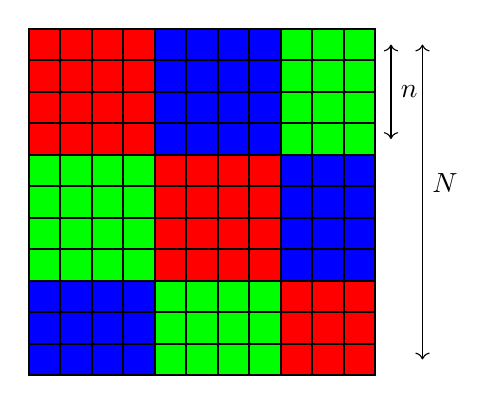
\begin{tikzpicture}
      [%%%%%%%%%%%%%%%%%%%%%%%%%%%%%%
          box/.style={rectangle,draw=black,thick, minimum size=.4cm},
          scale=0.4
      ]%%%%%%%%%%%%%%%%%%%%%%%%%%%%%%

  \foreach \x in {0,1,...,10}{
      \foreach \y in {0,1,...,10}
          \node[box] at (\x,\y){};
  }

  \foreach \x in {0,...,3}{
      \foreach \y in {7,...,10}
        \node[box,fill=red] at (\x,\y){};
  }

  \foreach \x in {4,...,7}{
      \foreach \y in {7,...,10}
        \node[box,fill=blue] at (\x,\y){};
  }

  \foreach \x in {8,...,10}{
      \foreach \y in {7,...,10}
        \node[box,fill=green] at (\x,\y){};
  }

  \foreach \x in {0,...,3}{
      \foreach \y in {3,...,6}
        \node[box,fill=green] at (\x,\y){};
  }

  \foreach \x in {4,...,7}{
      \foreach \y in {3,...,6}
        \node[box,fill=red] at (\x,\y){};
  }

  \foreach \x in {8,...,10}{
      \foreach \y in {3,...,6}
        \node[box,fill=blue] at (\x,\y){};
  }

  \foreach \x in {0,...,3}{
      \foreach \y in {0,...,2}
        \node[box,fill=blue] at (\x,\y){};
  }

  \foreach \x in {4,...,7}{
      \foreach \y in {0,...,2}
        \node[box,fill=green] at (\x,\y){};
  }

  \foreach \x in {8,...,10}{
      \foreach \y in {0,...,2}
        \node[box,fill=red] at (\x,\y){};
  }

  \draw[<->] (11,7) -- (11,10);
  \node[anchor=south west] at (11,8) {$n$};
  \draw[<->] (12,0) -- (12,10);
  \node[anchor=south west] at (12,5) {$N$};

  \end{tikzpicture}
\end{wrapfigure}

\noindent There is also research into applying loop tiling to the generated code, which is dividing the iterations of a loop into sub-regions where both temporal and spatial locality in memory can be exploited.\\
For example, a loop iterating over a 2D array of size $N \times N$, with Level 1 (L1) cache size of $n$ such that $n < N$ would benefit from dividing the array into squares of size at most $n \times n$, as long as this does not violate any data dependencies in the order of operations (see Figure \ref{fig:tile2D}). Doing so prevents values from being evicted from L1 cache prior to being needed again.
\par
Currently this has only been applied to OPS \cite{opstiling}, the precursor to OP2 \cite{opsmain}, which supports structured mesh solvers only. There does exist a 2019 paper \cite{slope} on automated loop tiling for unstructed meshes, and the issues posed by the need for indirect array accesses. A library provided which demonstrates the technique \cite{SLOPErep}, including a demo using the same \textit{airfoil} application used for this report.
\par
During this project it was suggested that applying loop tiling inside the JIT compilation stage could be a good extension, and would likely provide speedup, however unfortunately there was not sufficient time to reasonably expect the functionality to be finished.

\subsubsection{CUDA JIT Compilation}
Going in a different direction, the CUDA library does provide an interface for JIT compilation natively, which would allow for re-compilation without requiring a system call to \verb|make| for every loop kernel. System calls can be a significant bottleneck in some cases, and this problem would only compound for applications with a large number of parallel loops. Therefore, using the CUDA JIT compilation system would likely bring down the upfront cost of recompilation. For \textit{airfoil} this re-compile time is very low, it would not have much impact on the results gathered.

\subsubsection{Alternative Hardware Targets}
Finally, there are other hardware targets supported by OP2 which may be able to benefit from Just-In-Time compilation, and since the purpose of OP2 is to provide performance on multiple hardware platforms from a single application code any new optimisation which is found to improve performance, should also be ported to other platforms where it might be able to provide benefit. Any users who do not  primarly utilise Nvidia GPU hardware should benefit from the JIT compilation optimisation.

\subsection{Project Management}
\label{ss:pm}

% !TEX root =  ../report.tex

\section{Conclusion}
\label{s:conc}

This project was developed as an investigation into a new optimisation for the GPU code generation of the OP2 framework. As part of this investigation, an implementation of the technique was produced, and the results benchmarked to determine if the optimisation is able to provide benefit.
\par
The implementation was completed, producing the functionality for execution of JIT compiled code, and applied an optimisation made based on the inputs of the program, which can only be done at runtime - defining the constant values for the pre-processor.
\par
The results from this benchmarking were unfortunate, in that there was no benefit from the runtime, however it is important to draw the distinction that the defining of constants was not able to provide speedup, and not that JIT compilation as a technique does not have potential to speedup.
\par
It is likely that adding loop blocking as a runtime optimisation would produce better results, and adding this feature will have been made easier by the work completed for this project. It is unfortunate that there was not enough time to implement loop blocking, and benchmark it suffiently.
\par
Overall,


\newpage

%%TC:ignore
\printbibliography
% !TEX root =  ../report.tex


\appendixpage
\setcounter{section}{0}
\renewcommand{\thesection}{\Alph{section}}

\section{example}

%%TC:endignore

\end{document}
